\begin{prob}[3]\textbf{Newton's Method with Equality Constraints:}
\end{prob}
OBJECTIVE FUNCTION:
  \begin{eqnarray*}
    \mbox{minimize} & f(x) = \sum_{i=1}^{n} x_{i} \log x_{i}\\
    \mbox{subject to} & Ax = b
  \end{eqnarray*}
    with $\mathbf{dom} f = \mathbf{R}^{n}_{++}$ and $A \in \mathbf{R}^{p \times n}$,
  with $p < n$.
  
GRADIENT OF OBJECTIVE FUNCTION
\begin{eqnarray*}
\nabla f(x) &= \dfrac{\partial f(x)}{\partial x_{i}} \forall i = 1,2,\ldots,n\\
 &= 1 + \log x_{i}
\end{eqnarray*}
HESSIAN OF OBJECTIVE FUNCTION
\begin{eqnarray*}
\nabla^{2} f(x) =& \begin{cases}
\dfrac{\partial^{2} f(x)}{\partial x_{i}^{2}} & \mbox{if } i = j\\
\dfrac{\partial^{2} f(x)}{\partial x_{i}x_{j}} & \mbox{otherwise}\\
\end{cases}\\
 =& \mbox{\textbf{diag}}\left (\dfrac{1}{x_{i}} \right )
\end{eqnarray*}
Generate a problem instance with $n = 100$ and $p = 30$ by choosing $A$ randomly (checking that it has full rank), choosing $\widehat{x}$
  as a random positive vector (e.g., with entries uniformly distributed on
  $[0, 1]$) and the setting $b = A \widehat{x}$. (Thus, $\widehat{x}$ is
  feasible).

  Compute the solution of the problem using Infeasible start Newton Method.
  You can use initial point $x^{(0)} = \widehat{x}$ (to compare with the standard
  Newton Method), and also the initial point $x^{(0)} = \mathbf{1}$.
    \begin{figure}[H]
  \centering
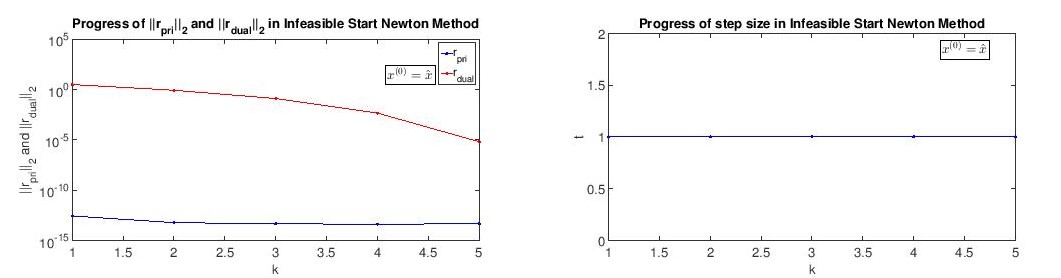
\includegraphics[width=\textwidth]{source/prob3/fig1}
%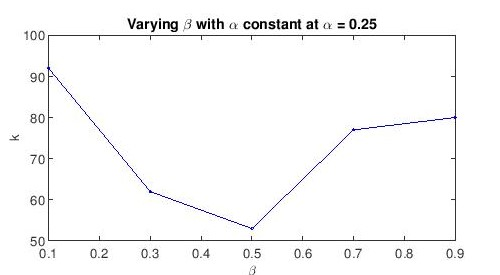
\includegraphics[width=5cm]{source/prob1/fig4}
\caption{Progress of $\vert \vert r_{pri} \vert \vert_{2}$, $\vert \vert r_{dual} \vert \vert_{2}$ and step size $t$ in the Infeasible Start Newton Method with $x^{0} = \widehat{x}$}
\end{figure}
  \begin{figure}[H]
  \centering
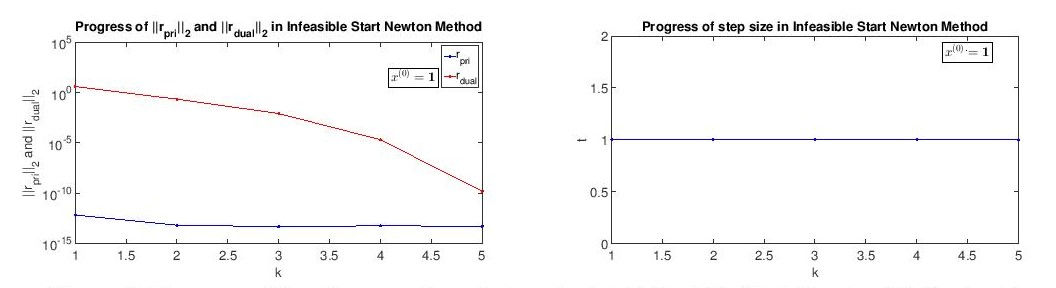
\includegraphics[width=\textwidth]{source/prob3/fig2}
%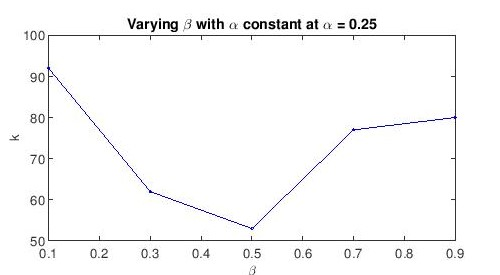
\includegraphics[width=5cm]{source/prob1/fig4}
\caption{Progress of $\vert \vert r_{pri} \vert \vert_{2}$, $\vert \vert r_{dual} \vert \vert_{2}$ and step size $t$ in the Infeasible Start Newton Method with $x^{0} = \mathbf{1}$}
\end{figure}
  \begin{figure}[H]
  \centering
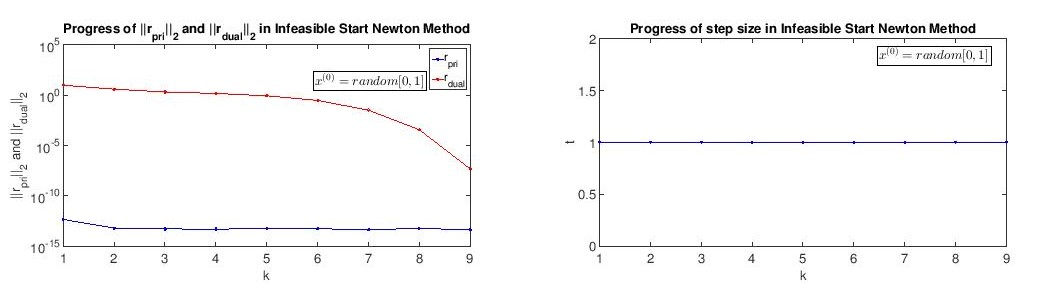
\includegraphics[width=\textwidth]{source/prob3/fig3}
%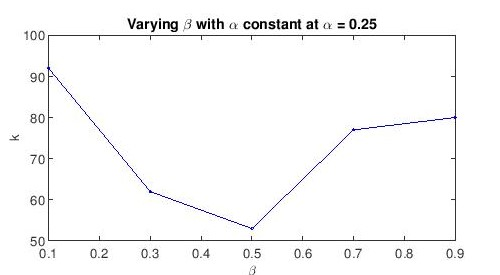
\includegraphics[width=5cm]{source/prob1/fig4}
\caption{Progress of $\vert \vert r_{pri} \vert \vert_{2}$, $\vert \vert r_{dual} \vert \vert_{2}$ and step size $t$ in the Infeasible Start Newton Method with $x^{0} = random[0,1]$}
\end{figure}